\section{Parametric studies based on the theoretical model}\label{sec:paramteric_studies_theory}
% Link to presentations: https://docs.google.com/presentation/d/1wqgJK7uDFDGoX8gyx2-JhnO8mZT51N1VH1RtNL-jhWA/edit#slide=id.ga69ead34aa_0_419

The basics of the existing theoretical model which describes the emittance growth in the presence of amplitude and phase noise in the $\CC$s in a synchrotron have been introduced in Chapter~\ref{Ch:CC_noise_theory}. Here, this theory is used to study the sensitivity of the noise-induced emittance growth on the $\CC$ voltage and rms bunch length. The objective of the study is to investigate if the uncertainty in the measurements of these two variables could explain the observed discrepancy of a factor $\sim$4 between measured emittance growth and the analytically predicted values (see Section~\ref{sec:meas_2018_vs_theory}).

The following parametric studies were performed for the experimental configuration of 2018: beam energy of 270\,GeV, vertical beta function of 73\,m (at the location of $\CC$2), and phase and amplitude noise of -111.4 and -115.7\,dBc/Hz respectively (Coast2-Setting2). The phase and amplitude noise are considered here independently, instead of the effective phase noise, due to the different dependence of the correction term (see Fig.~\ref{fig:correction_term_bunch_length}).

\subsection{Sensitivity to bunch length}\label{subsec:bunch_length_dependence}
Using Eqs.~\eqref{eq:dey_an} and~\eqref{eq:dey_pn} with the above mentioned parameters and CC votlage, $V_\mathrm{CC}$=1\,MV the normalised vertical emittance growth is computed as a function of different values of bunch lengths over a range from $10^{-3}$ to 2.5\,ns (expressed in $4\sigma_t$). The results are illustrated in Fig.~\ref{fig:sensitivity_bunch_length_theory_bunch1}. 

A clear dependence of the vertical emittance growth on the bunch length is observed. However, the dependence is strong for short bunches. In the regime of the measured bunch length during the CC experiment for bunch 1 (~1.6ns-2.0ns) the sensitivity to the bunch length is very small and cannot explain the factor of about 4 that was observed between measurements and simualtions in SPS $\CC$ tests in 2018.

% Plotting script: Requires python 3
% https://github.com/natriant/theoreticalModel_for_emitGrowth_due2CCNoise/blob/master/cmpt_GrowthDependence_on_BunchLength_003_for_thesis.py
\begin{figure}[!h]
    \centering         
    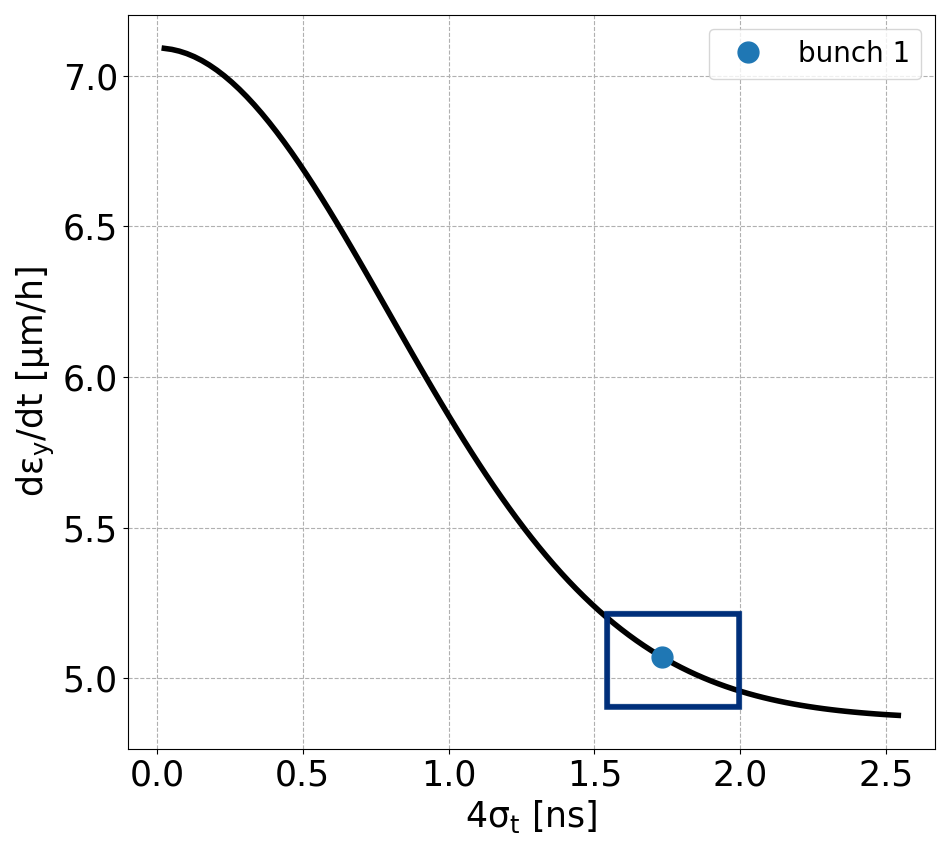
\includegraphics[width=0.7\textwidth]{images/Ch6/dey_vs_4sigmat_Coast2-Setting2_withBunches_v2.png}
        \caption{Vertical emittance growth for different bunch length values computed using the analytical formulas Eq.~\eqref{eq:dey_an} and~\eqref{eq:dey_pn} for the experimental configuration of 2018. The blue dot shows the average rms bunch length over all coasts in 2018. The blue box around it gives the upper and lower limits of its measurements.}
        \label{fig:sensitivity_bunch_length_theory_bunch1}
 \end{figure}


\subsection{Sensitivity to CC voltage}\label{subsec:bunch_length_dependence}

for the experimental configuration of 2018 

of the existing Vlasov theory for transverse coherent beam instabilities with first-order
chromaticity have been recapitulated in Section 2.2.3. Here, we extend this theory to account for the
beam dynamics effects introduced by nonlinear chromaticity. The chapter contains the work published
in Refs. [34, 76].



\newpage
\section{Benchmarking with different simulation software}
Benchmarking of theory with pyheadtail (one turn map) and Sixtracklib (element by element tracking).



\subsection{PyHEADTAIL}
- real CC element
- local vs global cc scheme
- How emittance is computed. No dipsersive contribution. studies vertical plane. \\
- It was verified in Sixtracklib simulations that the result from this simplified implementation is equivalent to the simulation with the true CC kick including phase noise.\\
- Need to say why in the simulations we have excitation of only the first betatron sideband. \\
\subsection{Sixtracklib}

Remember that in chapter 6 it was demonstrated that there is no visible difference on the cc rf noise induced emittance growth if the noise kicks are modeled as kicks on the moemntum or the real rf multiple + used in a global or local scheme.


pyheadtail vs sixtracklib: %https://docs.google.com/presentation/d/1rBVKGd9aBZTslaAHf48FdJkNPRyXtMF_T9XpEBlLE4c/edit#slide=id.g8ae11a254a_0_701

\section{Sensitivity to the non-linearities of the main SPS dipoles}
Simulation studies with sixtracklib

\section{Simulations using the measured noise spectrum}
Sixtracklib PyHEADTAIL and the exact machine paramters

\section{Sensitvity studies}
1. Sensitvity to how noisy is the noise spectrum
2. On the CC voltage
3. On the different bunch lengths. 

\section{b3b5b7 multiple errors}
Contribution of the non-linearities with sixtracklib.


All these factors were excluded as possible sources of the discrepancy.